% ****** Start of file apssamp.tex ******
%
%   This file is part of the APS files in the REVTeX 4.1 distribution.
%   Version 4.1r of REVTeX, August 2010
%
%   Copyright (c) 2009, 2010 The American Physical Society.
%
%   See the REVTeX 4 README file for restrictions and more information.
%
% TeX'ing this file requires that you have AMS-LaTeX 2.0 installed
% as well as the rest of the prerequisites for REVTeX 4.1
%
% See the REVTeX 4 README file
% It also requires running BibTeX. The commands are as follows:
%
%  1)  latex apssamp.tex
%  2)  bibtex apssamp
%  3)  latex apssamp.tex
%  4)  latex apssamp.tex
%
\documentclass[%
% reprint,
%superscriptaddress,
%groupedaddress,
%unsortedaddress,
%runinaddress,
%frontmatterverbose, 
%preprint,
%showpacs,preprintnumbers,
nofootinbib,
%nobibnotes,
%bibnotes,
 amsmath,amssymb,
aps,
%pra,
%prb,
%rmp,
%prstab,
%prstper,
%floatfix,
]{revtex4-1}

\usepackage{graphicx}% Include figure files
\usepackage{dcolumn}% Align table columns on decimal point
\usepackage{bm}% bold math
%\usepackage{hyperref}% add hypertext capabilities
%\usepackage[mathlines]{lineno}% Enable numbering of text and display math
%\linenumbers\relax % Commence numbering lines
\usepackage{subfigure}
\usepackage{amsthm}
\usepackage{amsmath}
%\usepackage{graphicx,caption,subcaption}
\graphicspath{{./Figs/}}
\usepackage{bbold}
\usepackage{tikz}
\usepackage{tkz-euclide}
\usepackage{adjustbox}
\usepackage{pst-solides3d}
\usetikzlibrary{matrix}
\usepackage{tikz-3dplot}
\usepackage[all,cmtip]{xy}

%\usepackage[showframe,%Uncomment any one of the following lines to test 
%%scale=0.7, marginratio={1:1, 2:3}, ignoreall,% default settings
%%text={7in,10in},centering,
%%margin=1.5in,
%%total={6.5in,8.75in}, top=1.2in, left=0.9in, includefoot,
%%height=10in,a5paper,hmargin={3cm,0.8in},
%]{geometry}
\theoremstyle{plain}% default
\newtheorem{thm}{Theorem}[section]
\newtheorem{lem}[thm]{Lemma}
\newtheorem{prop}[thm]{Proposition}
\theoremstyle{definition}
\newtheorem{defn}[thm]{Definition}
\newtheorem{exmp}[thm]{Example}
\theoremstyle{remark}
\newtheorem{rem}[thm]{Remark}
\usepackage{braket}


\def\nn{\nonumber}
\def\hom{\text{hom}(C,G)}
\def\homA{\text{hom}(C_A,G)}
\def\homtA{\text{hom}(C_{\tilde{A}},G)}
\def\homiA{\text{hom}(C_{\text{int}(A)},G)}
\def\homB{\text{hom}(C_B,G)}
\def\Hom{\text{Hom}}
\def\Z{\mathbb{Z}}
\def\H{\mathcal{H}}
\def\C{\mathbb{C}}

\def\ker{\text{ker}}
\def\im{\text{Im}}

\begin{document}

%\preprint{APS/123-QED}

\title{Ground State Degeneracy from Geometry in 3D}% Force line breaks with \\
%\thanks{A footnote to the article title}%

\author{J. P. Ibieta-Jimenez}
\email{pibieta@if.usp.br}

\author{M. Petrucci}%
 \email{marzia@if.usp.br}
 %\altaffiliation[Also at ]{Physics Department, XYZ University.}%Lines break automatically or can be forced with \\
\author{P. Teotonio-Sobrinho}%
 \email{teotonio@if.usp.br}
\affiliation{%
 Departamento de F\'isica Matem\'atica, Universidade de S\~ao Paulo\\ Rua do Mat\~ao Travessa R 187, CEP 05508-090, S\~ao Paulo, Brazil.
}%

\date{\today}% It is always \today, today,
             %  but any date may be explicitly specified

\begin{abstract}
We need an abstract....
\begin{description}
\item[Usage]
Secondary publications and information retrieval purposes.
\item[PACS numbers]
May be entered using the \verb+\pacs{#1}+ command.
\item[Structure]
You may use the \texttt{description} environment to structure your abstract;
use the optional argument of the \verb+\item+ command to give the category of each item. 
\end{description}
\end{abstract}

\pacs{Valid PACS appear here}% PACS, the Physics and Astronomy
                             % Classification Scheme.
%\keywords{Suggested keywords}%Use showkeys class option if keyword
                              %display desired
\maketitle



\section{\label{sec:intro}Introduction}
\begin{itemize}
\item Topological Order
\item Fractons
\item extensive degeneracy
\end{itemize}
The formalism developed in \cite{pramod} allows for the obtention of a large class of models where the bosonic degrees of freedom at vertices are coupled with gauge fields at links. Many such models can be got by the mere choice of the main ingredients, i.e., the gauge group $G$ and a $\mathbb{C}[G]$-module $(V_n, \mu)$. Aiming at a higher gauge theory interpretation, such models can be understood as a $0,1$-gauge theory. Since degrees of freedom are associated to both $0-cells$ (vertices) and $1-cells$ (links). In \cite{kazuothesis,ricardo} a very similar formalism is constructed for (3+1) topological phases using a $2$-group as the gauge group. This is, a $1,2$-gauge theory for topological phases of matter was constructed. In this case, degrees of freedom are associated to the $1-cells$ (links) and $2-cells$ (plaquettes). Taking these ideas into consideration, in \cite{higher} we constructed a Hamiltonian model for topological phases of matter in arbitrary dimensions. Furthermore, the notion of gauge group is promoted to a more general mathematical structure, that of a \textit{chain complex of abelian groups}. In this new framework, it can be shown \cite{higher} that the ground state degeneracy is a topological invariant of an abstract co-chain complex. In this sense, the ground state of such models is completely characterized and understood from the $0$-th cohomology group associated to such co-chain complex. Moreover, a theorem due to Brown \cite{Brown} relates this rather abstract cohomology group with the usual cohomology groups, enabling for a natural geometrical interpretation of the ground state subspace. 

Recently, we have found that by considering some of these fields as having only \emph{classical configurations}, the otherwise purely topological models now become sensitive to the geometry of the manifold upon which they are defined. This is showcased, as in the purely topological case, in the ground states of the Hamiltonian models, as we will show in the next section for a particular example. This fact has turned our attention to these new class of models that, we believe, are related to some other new findings in the topological phases of matter community. In particular, there is a strong interest in a new class of quantum states called \emph{fracton} phases \cite{chamon05,bravyi11,castelnovo12,haah11,bravyi13,yoshida13,vijay15,vijay16,vijay17,shirley17,rahul18}. Some characteristic of fracton phases include elementary excitations with restricted mobility and in some cases a ground state degeneracy that explicitly depends on the geometry of the manifold \cite{slagle17}. The latter has caught our attention as the higher gauge theories constructed in \cite{higher} can be modified to obtain a source of models with a geometrical dependence of the ground state degeneracy. The systematic construction of such models consists on restricting some $l$-constituents of the $n$-gauge configurations to be classical; This leads to equivalence classes of Hamiltonian models, some of which, have a geometrical dependence of the ground state degeneracy.  The construction of the models starting from the full higher gauge theories, the analysis of the unitary classes of Hamiltonians and the study of the geometrical models constitute the main contents of the Ph.D. research project. In this sense, the main objective of the research project is to characterize the topological and geometrical phases coming from the procedure of partially freezing the degrees of freedom. This endeavor is partially achieved since the construction of the models and their characterization with respect to the appearance of geometrical phases or not is known, as we will show in the next section. There are, however, some details that have to be concealed before considering the project as finished, they include:
\begin{itemize}
\item A Proof that the geometrical states are indeed the ground states of such Hamiltonians.
\item A brief study of the excited states, paying special attention to the mobility restrictions that appear in fracton phases.
\item To fit the description of the models into the formalism developed in \cite{higher}.
\end{itemize}

\section{Geometric Quantum Models }\label{sec:QModels}

In this section we define two quantum models whose ground states exhibit dependence on geometric features of the underlying lattice. We begin with a 2-dimensional model which will be used as a warm up for the 3-dimensional version that comes next.

\subsection{2D Geometric Quantum Model }\label{sec:2Dmodel}

\subsection{3D Geometric Quantum Model }\label{sec:3Dmodel}

Roughly speaking, the model consists in a 1-gauge theory of the type considered in \cite{higher,higher-ent} whose Hilbert space gets now decorated by classical 2-gauge configurations, as we will see. So, we consider a 1-gauge theory defined over an arbitrary \(d\)-dimensional lattice that can come from a simplicial complex \(K=\bigcup_{n=0}^d\,K_n\), for instance. More precisely, we will associate \(G_1\)-valued degrees of freedom to the links \(l \in K_1\) of the lattice or, the local Hilbert spaces \(\H_l\) are spanned by basis elements \(\{\ket{g},\, g \in G_1\}\). The global Hilbert space is taken to be the tensor product of these local spaces, i.e., $\mathcal{H} :=\bigotimes_{l \in K_1} \H_l$. Additionally, we will consider to the where $\xi: C_2 \rightarrow  G_2$ is a classical configuration (coloring) of degrees of freedom at plaquettes $p \in K_2$ taking values in the Abelian group $G_2$. Moreover, we consider the group homomorphism, $\partial: G_2 \rightarrow G_1$.
The Hamiltonian of the model is given by:
\begin{equation}\label{eq:Hgeo}
H(\xi) = - \sum_{p\in K_2} B_p(\xi) - \sum_{v \in K_0} A_v,
\end{equation}
where the $A_v$ is the usual gauge transformation of a 1-gauge theory, eq. (\ref{eq:Av1G}).On the other hand, the holonomy measurement operator gets modified because of the classical configurations living at plaquettes of the complex. The operator will be, instead, similar to its 2-gauge counterpart, of eq. (\ref{eq:Bp2G}), i.e.,
\begin{align}\label{eq:Bp2G}
 B_p(\xi) \quad \vcenter{\hbox{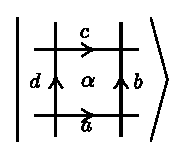
\includegraphics[scale=0.65]{Bp2Gket1.eps}}}\ &= \delta(a+b-c-d,\partial(\alpha))\ \vcenter{\hbox{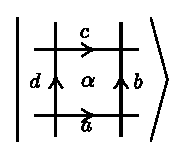
\includegraphics[scale=0.65]{Bp2Gket1.eps}}},
\end{align}
notice that in this case the 2-gauge parameter, $\alpha \in G_2$ is now fixed by the classical configuration $\xi(p)=\alpha$, and it is not dynamical as in the full 2-gauge theory (cf. \S \ref{sec:2gauge}). 

The model can be thought of as being a 2-gauge theory whose plaquette degrees of freedom are now fixed. The fixing of the 2-gauge fields is carried out via the $\xi$ maps. Thus, we are actually dealing with a family of Hamiltonians parametrized by the $\xi$ maps. The role that was being played by the 2-gauge transformation, eq. (\ref{eq:Av2G}), is now split into two transformations that divide the family Hamiltonians into equivalence classes. 

\begin{defn}\label{def:coltrans}
Given a 1-cell (link) $l \in K_1$ and an element $\beta \in G_2$, we define the \emph{color transformation} $T_l(\beta):\xi \rightarrow \xi^{\prime}$, where $\xi$ and $\xi^{\prime}$ are two 2-gauge classical configurations that differ by $T_l(\beta)$ as follows:

\begin{figure}[h!]
\centering
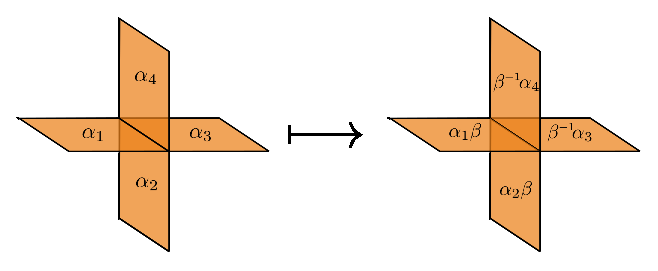
\includegraphics[scale=0.8]{color2G.eps}
\label{fig:coltrans}
\end{figure}

This is, the colorings of the faces around the link $l \in K_1$ are all transformed by the parameter $\beta$ according to the orientations. 
\end{defn}
It is important to emphasize that the above transformation is NOT a 2-gauge transformation, as it is actually mapping between different Hamiltonians. So, in general, for two different colorings $\xi$ and $\xi^{\prime}$ their corresponding Hamiltonians are different, i.e., $H(\xi)\neq H(\xi^{\prime})$. However, if the two colorings, $\xi$ and $\xi^{\prime}$, differ from one another by a color transformation $T_l(\beta)$ (or a sequence of them), it can be shown that the two corresponding Hamiltonians are unitarily equivalent. To achieve this goal, we define the following unitary transformation.
\begin{defn}\label{def:unitrans} Let $l \in K_1$ be an arbitrary 1-cell, a parameter $\beta \in G_2$ and a basis element $\ket{g}\in \mathcal{H}_l$, $g \in G_1$; The \emph{unitary} transformation $U_l(\beta):\mathcal{H}_\xi \rightarrow \mathcal{H}_{\xi^{\prime}}$ is given by:
\[U_l(\beta)\ket{g}=\ket{\partial(\beta)g},\]
where $\partial:G_2 \rightarrow G_1$.
\end{defn}

It is worthwhile pointing out that, in the above definition, both $\mathcal{H}_\xi$ and $\mathcal{H}_{\xi^{\prime}}$ are actually the same Hilbert space, we just write the subscript to highlight the fact that the transformation corresponds to a mutation of colorings from $\xi$ to $\xi^{\prime}$. 
\begin{prop} Let $\xi$ and $\xi^{\prime}$ are two colorings, connected by $T_l(\beta)$ for a given $l \in K_1$. Then, the two Hamiltonians $H(\xi)$ and $H(\xi^{\prime})$ are unitarily equivalent, this is,
\[U_l^{-1}(\beta)H(\xi^{\prime})U_l(\beta) = H(\xi).\]
\end{prop}
\begin{proof}
To show that the above proposition is true, we only need to prove the following:
\[U_l^{-1}(\beta)B_p(\xi^{\prime})U_l(\beta) = B_p(\xi),\]
for all plaquettes $p \in K_2$ adjacent to the link $l$, or more precisely, that have the link $l$ as a boundary. Which follows straightforwardly from applying the definition \ref{def:unitrans} and the definition of the plaquette operator of eq. (\ref{eq:Bp2G}).
\end{proof}
From this unitary equivalence we are able to identify the different equivalence classes of models.
We now turn into an specific example in order to see the geometrical properties of the models. 

\begin{exmp}
We define the model over a lattice that can come from a simplicial complex of a 3 dimensional manifold $\mathcal{M}$, homeomorphic to $S_2 \times I$, such that it has a shortest (dual) path $\gamma$ between the two boundaries:
\begin{figure}[h!]
\centering
    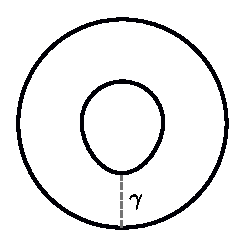
\includegraphics[scale=0.7]{shortest.eps}

\end{figure}

The requirement of having this shortest path is arbitrary and we make this assumption in order to precisely exhibit the main feature of the model. Furthermore, we consider the groups as being $G_1=G_2=\mathbb{Z}_2=\{1,-1\}$ together with the group homomorphism $\partial:\mathbb{Z}_2 \xrightarrow{id} \mathbb{Z}_2$. So we're dealing with a $\mathbb{Z}_2$ 1-gauge theory with classical fields at faces taking values in $\mathbb{Z}_2$, as well. Consequently, the Hilbert space of the model is $\mathcal{H}:=\bigotimes_{l}\mathbb{C}[\mathbb{Z}_2]_l$; An arbitrary basis state $\ket{\psi} \in \mathcal{H}$ consists of spins configurations that will be represented by red (dual) surfaces or the lack of them. We choose this representation as it is best suited for our purpose of exhibiting the ground state in terms of surfaces and strings. For instance, the following configuration:
\begin{figure}[h!]
\centering
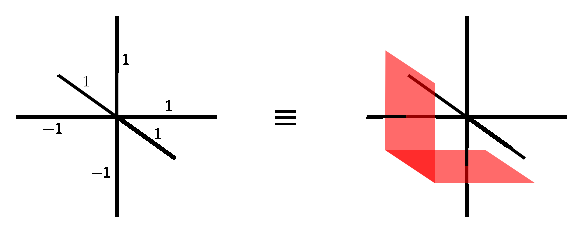
\includegraphics[scale=0.8]{graphstate.eps}
\end{figure}

where the $\ket{-1}$ configurations are represented by dual red surfaces. On the same spirit, we will also use a graphical notation for the coloring of the Hamiltonian  represented in the lattice as green (dual) strings, this is, strings going through faces of the lattice; We would like to emphasize that in this case, we are thinking of the maps $\xi:C_2 \rightarrow G_2$ as decorating the lattice with (dual) strings; These strings are NOT representations of states as the local Hilbert spaces live on the links of the lattice only, for instance, the two possible color configurations on a plaquette are shown in Fig.\ref{fig:plaqconfig}.

\begin{figure}[h!]
\centering
\subfigure[]{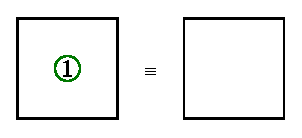
\includegraphics[scale=0.65]{col1.eps}}\hspace{30pt}
\subfigure[]{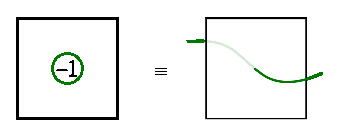
\includegraphics[scale=0.65]{col2.eps}}
\caption{\label{fig:plaqconfig} The two possible colorings at a single plaquette are shown.}
\end{figure}

The vertex operator, $A_v$, that implements local gauge transformations is composed of two parts: 
\[A_v=\dfrac{1}{2}(A_v^{1}+A_v^{-1}),\]
where $A_v^1=\mathbb{1}$ and the action of $A_v^{-1}$ is to flip the configurations from $\ket{1}$ to $\ket{-1}$ and vice versa, around the vertex in question. Concerning our representation of surfaces, the action of local gauge transformations is to either create red spheres or to modify surfaces by isotopy. 

The plaquette operator, $B_p(\xi)$, projects into the "flat"-holonomy subspace of $\mathcal{H}$. Notice that, since they depend on the coloring $\xi$, the configurations that are considered "flat" depend now on the coloring of the lattice. When the coloring is trivial, this is, $\xi(p)=1,\ \forall p \in K_2$, the plaquette operator favors configurations with and even number (or zero) of surfaces around a plaquette. A consequence of this is that, overall, the "flat" sector corresponds to configurations of closed surfaces in the bulk that can open in the each of the boundaries of $\mathcal{M}$. We will refer to this case ($\xi(p)=1,\ \forall p \in K_2$) as \emph{trivial} as it corresponds to defining the Toric Code \cite{Kitaev1} on $\mathcal{M}$. There are, however, colorings that are different from the trivial one, where some or many plaquettes might have a $-1$ coloring attached to it. In the case a particular plaquette $p \in K_2$ has such a coloring, the corresponding plaquette operator will project states different from the trivial case. For instance, the following state:
\begin{align*}
 B_p \quad \vcenter{\hbox{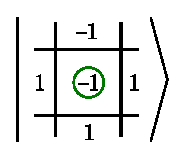
\includegraphics[scale=0.65]{Bket1.eps}}}\ = \delta(1(-1)11,-1)&\  \vcenter{\hbox{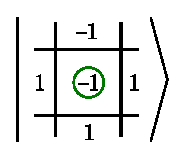
\includegraphics[scale=0.65]{Bket1.eps}}},\\
 = &\vcenter{\hbox{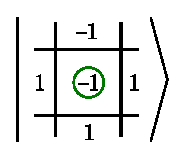
\includegraphics[scale=0.65]{Bket1.eps}}},
\end{align*}
the state has a single link configuration with $\ket{-1}$ yet the plaquette operator is giving a eigenvalue of 1. This particular configuration would not be considered as "flat" in the trivial theory. In our graphical notation, this state would look like:
\begin{figure}[h!]
\centering
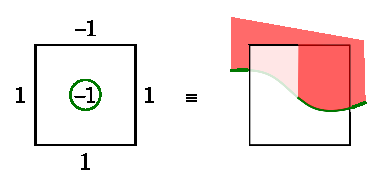
\includegraphics[scale=0.8]{graph2.eps}
\end{figure}
\end{exmp}
The above shows that open surfaces in the bulk are allowed, as long as they end on a green (dual) string, this modifies the dynamics of the model with respect to the trivial case and in particular, the nature of the ground states. To understand this let us look at the different unitary classes of Hamiltonians there are. Hamiltonian of eq.(\ref{eq:Hgeo}) depends on the way the lattice is decorated, given by the maps $\xi$. In principle, different colorings of the lattice give rise to different models; This is true, up to equivalence classes. 
The reason is the existence of both the color transformation of Def. \ref{def:coltrans} and the unitary transformation of Def.\ref{def:unitrans}, to see this let us study the action of both transformations on the colorings and the states. By looking at Def.\ref{def:coltrans} we note that the color transformations are labeled by \(G_2= \mathbb{Z}_2\); Therefore, for a given link \(l \in K_1\) there are two elementary color transformations, namely, \(T_l(1)= \text{id}\) and \(T_l(-1)\) that flips the configurations at plaquettes around \(l\), as shown in Def. \ref{def:coltrans}. Thus, the only non trivial action of the color transformation is given by \(T_l(-1)\) and can thought of as either creating a closed (dual) string around the link \(l\) or extending an existing string by local isotopy, as shown in Fig.(\ref{fig:coltrans}).
With this information we are able to explore the equivalence classes of Hamiltonians. The color transformation can only add closed dual strings or extend existing ones by isotopy; Also, considering that closed dual strings on the bulk can be opened at the two boundaries of \(\mathcal{M}\) it is nor difficult to realize that there are two unitary equivalence classes of Hamiltonians.

\begin{figure}[h!]
\centering
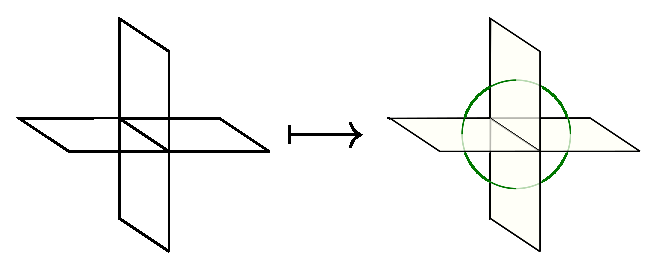
\includegraphics[scale=0.6]{coltrans.eps}
\caption{\label{fig:coltrans}Color transformation around a link.}
\end{figure}

\textbf{Class 1.-} This class corresponds to the trivial coloring model, i.e., all colorings that are unitarily equivalent to the model with trivial coloring. The equivalence class corresponds to having an even number of dual strings connecting the two boundaries, as it is shown in Fig. \ref{fig:class1}. This class of models correspond to defining the Toric Code on the manifold \(\mathcal{M}\). We wont dwell onto the details of this class of models since they are all known as they correspond to the usual topological models. A detailed description will be found on \cite{pablo}.
\begin{figure}[h!]
\centering
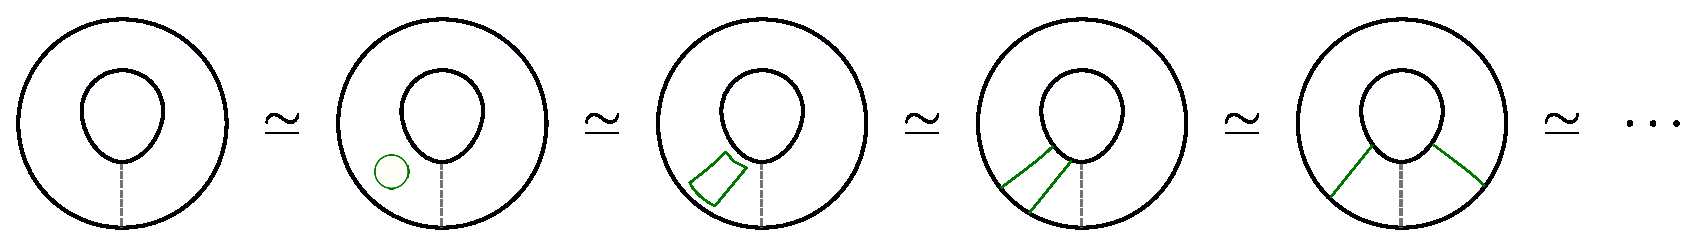
\includegraphics[scale=0.55]{class1.eps}
\caption{\label{fig:class1}Some equivalent colorings of class 1 are shown.}
\end{figure}

\textbf{Class 2.-} This class consists on all lattice colorings that have an odd number of strings connecting the two boundaries of \(\mathcal{M}\), as shown in Fig.\ref{fig:class2}. This is the class of models that we are interested in, consequently we will give a preliminary analysis of the ground state subspace of such models. First of all, we know is sufficient to take a representative of the class and we will work with the coloring with one single dual string connecting the two surfaces.
\begin{figure}[h!]
\centering
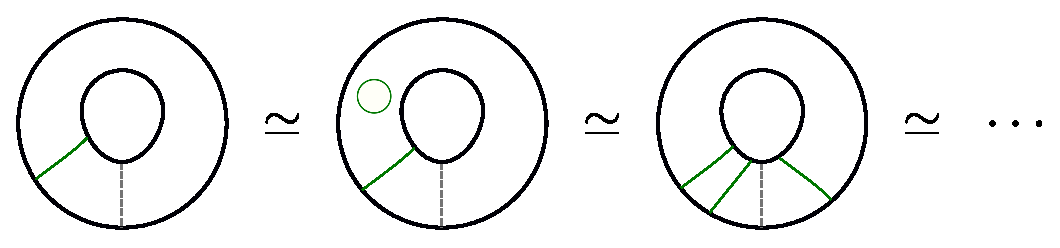
\includegraphics[scale=0.55]{class2.eps}
\caption{\label{fig:class2}Some equivalent colorings of class 2 are shown.}
\end{figure}

To study the ground state of the model we first notice that all plaquettes being crossed by the string will project to the holonomy value of \(-1\). Therefore, if we take the coloring of the representative in Fig.\ref{fig:class2} and consider the seed state with \(\ket{1}\) at every link, the following state:
\[\ket{\psi}= \prod_v A_v\ \ \vcenter{\hbox{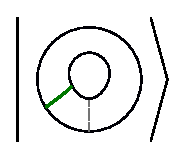
\includegraphics[scale=0.65]{ket1.eps}}}\ ,\]
has an energy proportional to the length\footnote{By length we mean the number of plaquettes being crossed by the string.}, \(l_p\), of the string. This can be seen from the eigenvalues of the plaquette operators affected by the coloring:
\[B_p\ \ \vcenter{\hbox{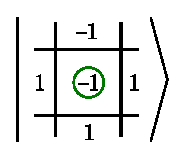
\includegraphics[scale=0.65]{Bket1.eps}}} = \delta(1111,-1)\ \ \vcenter{\hbox{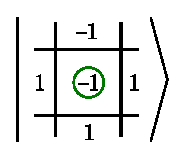
\includegraphics[scale=0.65]{Bket1.eps}}}=0\ ,\]
therefore evaluating the Hamiltonian operator on this state we obtain:
\begin{equation}\label{eq:Epsi}
H\ket{\psi}=-(N_v -(N_p - l_p))\ket{\psi},
\end{equation}

where \(N_v= |K_0|\) and \(N_p=|K_2|\) are the number of vertices and plaquettes, respectively.
hence, it is clear that the energy of such a state depends linearly on the length of the string. Naturally, arises the question of whether it exists a state with less energy than \(\ket{\psi}\). We recall that the minimum energy in the topological case (class 1) is \(E_0=-N_v - N_p\), thus we can also ask if whether this is the energy minimum for the Hamiltonians of class 2. The answer to both questions is obtained by looking at the details of \(\mathcal{M}\), recall that the lattice we over which the model is defined has a shortest dual path \(\gamma\) that joins the two surfaces. Thus, if we consider the following state,
\[\ket{\psi_0}= \prod_v A_v \ \ \vcenter{\hbox{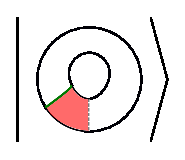
\includegraphics[scale=0.65]{ket2.eps}}}\ ,\]
that consists on a red surface extending from the coloring string to the shortest path. Evaluating the Hamiltonian operator over this state we obtain,
\begin{equation}\label{eq:Epsi0}
H\ket{\psi_0}=-(N_v -(N_p - \gamma_p))\ket{\psi_0}, 
\end{equation}
now, we  know that \(\gamma_p  < l_p\) for any dual string length \(l_p\). Therefore,  \(\ket{\psi_0}\) is the state with least energy in \(\mathcal{H}\).
We want to stress that no matter what representative of the class of Hamiltonians we choose, the ground state will still perform the same task, this is, to find the shortest path between the two surfaces. Notice that, to localize this path it is enough to act with plaquette operators and look for the ones that get excited. As one can see in eqns. (\ref{eq:Epsi}) and (\ref{eq:Epsi0}), the energy of these states is bigger than the ground state energy of the Hamiltonians in class 1, this is due to the existence of a single dual string on the lattice. To understand this let us look at the concrete action of the coloring $\xi$ on the dynamics of the models; The dual string modifies the plaquette operators on its path making them project to the $-1$ sector, this can be thought of as condensing flux excitations at these plaquettes. However, flux excitations in the (trivial) theory always come in pairs, concretely pairs of dual strings (up to gauge transformations). Then by condensing one of the strings at the modified plaquettes there is one single dual string of excitations left "free". The ground state of the models consist on placing this "free" dual string at the shortest (dual) path from one inner to the outer surfaces, thus minimizing the energy of the state. 

We see that even on the simplest example we get rich new behavior both for the ground states and the excited states. The geometric property of the ground state makes us place these models into what is known as fracton phases \cite{chamon05,rahul18}. Moreover, the procedure of making classical some degrees of freedom  of a higher gauge theory we have a plethora of models with similar phenomena. The construction can be carried out for arbitrary dimensions and gauge fields. The goal of the Ph.D. thesis manuscript is to condense all these models and phenomena in a rigorous and concrete way. To do so, we sketch the future work schedule that will be followed until the finishing of the manuscript.

 
\section{Geometric Ground State Degeneracy}\label{sec:G-GSD}
\subsection{2D Model}
\subsection{3D Model}

\section{Conclusions}\label{sec:Remarks}

\appendix






\section{Trace of Local Operators}\label{sec:app2}
In this appendix we show how taking the partial trace of the ground state projector, or any product of projection operators of the theory, implies in Eq.(\ref{eq:rhoA1}). This is, we show that the local projectors \(A_{n,x}\) and \(B_{n,x}\) are traceless unless they are trivial (equal to the identity operator).

We begin by writing the density matrix, \(\rho\), using the local decomposition of \(\mathcal{A}_0\) and \(\mathcal{B}_0\) (see \cite{higher} for a detailed account on this). The local decomposition yields:
\begin{align*}
\mathcal{A}_0 = \prod_{n=0}^{d} \prod_{x\in K_n} A_{x}, \; \text{and}\quad \mathcal{B}_0 = \prod_{n=0}^{d} \prod_{x\in K_n} B_{x},
\end{align*}
such that the density matrix of Eq.(\ref{eq:rho}) can be written as:
\begin{align*}
\rho = \dfrac{1}{GSD} \left(\prod_{n=0}^{d} \prod_{x\in K_n} A_{x}\right)\left(\prod_{n=0}^{d} \prod_{x\in K_n} B_{x}\right),
\end{align*}
this form is convenient for taking the partial trace as the operators are now localized at simplices $x \in K_n$ for $0\leq n \leq d$, this allows for the identification of the operators that act exclusively on region $A$ from the operators that act on both $\partial(A)$ and $B$, in order to get the terms that survive the partial trace.
In this sense, the reduced density matrix is written as:
\begin{align}\label{eq:rhoAlocal}
\rho_A = \text{Tr}_B(\rho)= \;\text{Tr}_B\left(\prod_n \prod_{x \in K_n}A_{x}\prod_{y \in K_n}B_{y}\right).
\end{align}
Before going onto the calculation of the above partial trace, we will prove a property that will let us evaluate the partial trace rather straightforwardly.


\begin{prop}\label{prop:traceless}
Let \(x,y \in K_n\), be $n$-simplices for \(0\leq n\leq d\). The local operators, \(A_{x}, B_{y}:\mathcal{H}\rightarrow\mathcal{H}\), are traceless unless they act  trivially (as the identity operator \(\mathbb{1}_\mathcal{H}\)).
\end{prop}
\begin{proof}
Let \(\{\ket{f}\}\) be a basis of $\mathcal{H}$, with \(f \in \hom^0\). We start by taking the trace of the local gauge transformations:
\begin{align*}
\text{Tr}\left(A_{x}\right) = & \sum_{f} \bra{f} A_{x} \ket{f} = \dfrac{1}{\left|G_{n+1}\right|}\sum_{f}\, \sum_{g \in G_{n+1}} \bra{f} A_{e[x,g]} \ket{f}.
\end{align*}
From Definition \ref{def:AopBop}, the action of \(A_{n,x}\) on a basis state consists in general on a shift of basis elements, which yields:
\begin{align*}
\text{Tr}\left(A_{x}\right) =&  \dfrac{1}{\left|G_{n+1}\right|}\sum_{f}\, \sum_{g \in G_{n+1}} \bra{f}  \ket{f+ \delta^{-1}(e[x,g])}.
\end{align*}
From the last expression it is clear that the only non-null term in the sum occurs only when \(g=e \in G_{n+1}\), the identity element. Thus, we have:
\begin{align*}
\text{Tr}\left(A_{n,x}\right) =& \dfrac{\text{Tr}\left(\mathbb{1}\right)}{\left|G_{n+1}\right|} = \dfrac{\dim(\mathcal{H})}{\left|G_{n+1}\right|}.
\end{align*}
 Similarly, for the trace of local holonomy measurement operators,\(B_{n,y}\), we have:
\begin{align*}
\text{Tr}\left(B_{y}\right) = & \sum_{f} \bra{f} B_{x} \ket{f} = \dfrac{1}{\left|G_{n-1}\right|}\sum_{f}\, \sum_{r \in \hat{G}_{n-1}} \bra{f} B_{\hat{e}[y,r]} \ket{f}. 
\end{align*}
Using Definition \ref{def:AopBop} the above expression can be written as:
\begin{align*}
\text{Tr}\left(B_{y}\right) =\;  \dfrac{1}{\left|G_{n-1}\right|}\sum_{f}\, \sum_{r \in \hat{G}_{n-1}} \chi_r\left({f_n(y)}\right)\braket{f|f}\;
=\;  \dfrac{1}{\left|G_{n-1}\right|}\sum_{f}\, \sum_{r \in \hat{G}_{n-1}} \chi_r\left({f_n(y)}\right)\chi_{\hat{e}}\left({f_n(y)}\right)\braket{f|f},
\end{align*}
where in the last line we used the fact that \(\chi_{\hat{e}}(g)=1, \, \forall g \in G_{n-1}\) and \(\hat{e} \in \hat{G}_{n-1}\), the trivial representation. From the orthogonality relations of characters \cite{hall, barut,serre, james}, we note that:
\begin{align*}
\sum_{f}\chi_r\left({f_n(y)}\right)\chi_e\left({f_n(y)}\right) = \delta(e,f_n(y)), 
\end{align*}
which implies that the trivial representation term is the only one that has non-zero trace, since it acts as the identity operator.
\begin{align*}
\text{Tr}\left(B_{y}\right) = & \dfrac{\left|\mathcal{H}\right|}{\left|G_{n-1}\right|}
\end{align*}
\end{proof}
 This result can naturally be extended to products of such operators to show that the only term that survives the trace is the one that acts trivially. This allows us to express  the reduced density matrix, \(\rho_A\) of Eq.(\ref{eq:rhoAlocal}) in terms of operators that act only in region \(A\). 
 
 In this case,  Proposition \ref{prop:traceless} implies that any operator (or product of several) that is different from \(\mathbb{1}_B\), the identity operator in \(\mathcal{H}_B\), will have vanishing trace. This, in turn, tells us about the nature of the operators that survive the trace; In particular, local gauge transformations \(A_{x}\) will survive the trace if and only if \(x \in K_{n,\tilde{A}}\), where \(\tilde{A}\) is the interior of \(A\) \footnote{Local gauge transformations are labeled by simplices \(x \in K_n\) and they act on the gauge fields at the co-boundary, \(\partial^{\ast}(x)\). In particular, gauge transformations located at \(x \in K_{n,{\partial(A)}}\), the boundary of \(A\), also act on \(B\). Thus, they do not contribute to the trace.} as in Def. \ref{def:intA}. On the other hand, local holonomy measurement operators \(B_{y}\) will survive the trace if and only if \(y \in K_{n,A}\) which corresponds to the entire region $A$. Consequently, the reduced density matrix is:
\begin{align*}
\rho_A =\text{Tr}_B(\mathbb{1}_B) \prod_{n} \prod_{x \in K_{n,\tilde{A}}}A_{x}\prod_{y \in K_{n,A}}B_{y} .
\end{align*}  
From which we write Eq. (\ref{eq:rhoA1}).

\bibliographystyle{apsrev4-1}
\bibliography{bib.bib}
\end{document}
%
% ****** End of file apssamp.tex ******
